%% Direttive TeXworks:
% !TeX root = ./summary.tex
% !TeX encoding = UTF-8 Unicode
% !TeX spellcheck = it_IT
% !TeX program = arara
% !TeX options = --log --verbose --language=it "%DOC%"

% arara: pdflatex:      { interaction: nonstopmode, shell: yes }
% arara: pdflatex:      { interaction: nonstopmode, shell: yes }
% arara: pdflatex:      { interaction: nonstopmode, synctex: yes, shell: yes }

\documentclass{llncs}

\usepackage{a4wide}

%%%%%%%%%%%%%%%%%%%%%%%%%%%%%%%%%%%%%%%%%%%%%%%%%%%%%%%%%%%
%% package sillabazione italiana e uso lettere accentate
\usepackage[T1]{fontenc}
\usepackage{textcomp}
\usepackage[utf8]{inputenc}
\usepackage[english,italian]{babel,varioref}
\usepackage{lmodern}
\usepackage[%
  strict,
  autostyle,
  english=american,
  italian=guillemets
]{csquotes}
%%%%%%%%%%%%%%%%%%%%%%%%%%%%%%%%%%%%%%%%%%%%%%%%%%%%%%%%%%%%%

\usepackage{fancyvrb}

%% Genera un file report.xmpdata con i dati di titolo e autore per il formato PDF/A %%
\begin{VerbatimOut}{\jobname.xmpdata}
  \Title{Laboratorio di Sistemi Software --- Breve presentazione del tema finale}
  \Subject{Realizzazione di un sistema per l'individuazione e rimozione di una bomba dalla hall di un aeroporto tramite robot controllato da remoto.}
  \Author{Niccolò Maltoni}
  \Copyright{Questo documento è fornito sotto licenza Apache License, Version 2.0}
  \CopyrightURL{https://opensource.org/licenses/Apache-2.0}
\end{VerbatimOut}

\usepackage{relsize, etoolbox}
\AtBeginEnvironment{foreigndisplayquote}{\smaller}

\usepackage{indentfirst}
\usepackage{xurl}
\usepackage{setspace}
\usepackage{xspace}

\makeatletter

%%%%%%%%%%%%%%%%%%%%%%%%%%%%%% User specified LaTeX commands.
\usepackage{manifest}

\makeatother

\usepackage{natbib}
\usepackage{xcolor}

\usepackage{graphicx}
\DeclareGraphicsExtensions{.eps, .pdf, .jpg, .tif, .png} % chktex 26

\usepackage{subcaption}
\usepackage{float}

\usepackage[savemem]{listings}
\usepackage{listingsutf8}

\definecolor{dkgreen}{rgb}{0,0.6,0}
\definecolor{gray}{rgb}{0.5,0.5,0.5}
\definecolor{mauve}{rgb}{0.58,0,0.82}

\lstset{
  extendedchars=true,
  inputencoding=utf8/latin1,
  frame=single,
  captionpos=b,
  language=Java,
  showspaces=false,
  showtabs=false,
  showstringspaces=false,
  columns=flexible,
  basicstyle={\small\ttfamily},
  numbers=none,
  numberstyle=\tiny\color{gray},
  keywordstyle=\color{blue},
  commentstyle=\color{dkgreen},
  stringstyle=\color{mauve},
  breaklines=true,
  breakatwhitespace=true,
  keepspaces=true,
  numbersep=5pt,
  tabsize=2
}

\lstdefinelanguage{qa}{
  basicstyle=\ttfamily\scriptsize,
  numbers=left,
  numberstyle=\scriptsize,
  stepnumber=1,
  numbersep=8pt,
  tabsize=2,
  showstringspaces=false,
  breaklines=true,
  breakatwhitespace=true,
  keywordstyle=\color{mauve}\bfseries,
  commentstyle=\color{dkgreen},stringstyle=\color{blue},
  morekeywords={System,Event,Dispatch,Context,QActor,Rules,State,%
      demo,whenMsg,whenEvent,onMsg,onEvent,transition,stopAfter,%
      whenTime,resumeLastPlan,initial,finally,javaRun,println,%
      emit,forward,do},
  otherkeywords={:,->,-m,;,.,\,,[,],:-},
  morestring=*[d]{"}, % chktex 18
  morecomment=[l]{//},
  morecomment=[s]{/*}{*/}
}

\newcommand{\java}{\textsf{Java}}
\newcommand{\contact}{\emph{Contact}}
\newcommand{\corecl}{\texttt{corecl}}
\newcommand{\medcl}{\texttt{medcl}}
\newcommand{\msgcl}{\texttt{msgcl}}
\newcommand{\android}{\texttt{Android}}
\newcommand{\dsl}{\texttt{DSL}}
\newcommand{\jazz}{\texttt{Jazz}}
\newcommand{\rtc}{\texttt{RTC}}
\newcommand{\ide}{\texttt{Contact-ide}}
\newcommand{\xtext}{\texttt{XText}}
\newcommand{\xpand}{\texttt{Xpand}}
\newcommand{\xtend}{\texttt{Xtend}}
\newcommand{\pojo}{\texttt{POJO}}
\newcommand{\junit}{\texttt{JUnit}}

\newcommand{\action}[1]{\texttt{#1}\xspace}
\newcommand{\code}[1]{{\small{\texttt{#1}}}\xspace}
\newcommand{\codescript}[1]{{\scriptsize{\texttt{#1}}}\xspace}

\newcommand{\requirement}[1]{\hypertarget{req:#1}{\textcolor{blue}{#1}}}
\newcommand{\requirementref}[1]{\hyperlink{req:#1}{\textcolor{blue}{#1}}}

% Cross-referencing
\newcommand{\labelsec}[1]{\label{sec:#1}}
\newcommand{\xs}[1]{\sectionname~\ref{sec:#1}}
\newcommand{\xsp}[1]{\sectionname~\ref{sec:#1} \onpagename~\pageref{sec:#1}}
\newcommand{\labelssec}[1]{\label{ssec:#1}}
\newcommand{\xss}[1]{\subsectionname~\ref{ssec:#1}}
\newcommand{\xssp}[1]{\subsectionname~\ref{ssec:#1} \onpagename~\pageref{ssec:#1}}
\newcommand{\labelsssec}[1]{\label{sssec:#1}}
\newcommand{\xsss}[1]{\subsectionname~\ref{sssec:#1}}
\newcommand{\xsssp}[1]{\subsectionname~\ref{sssec:#1} \onpagename~\pageref{sssec:#1}}
\newcommand{\labelfig}[1]{\label{fig:#1}}
\newcommand{\xf}[1]{\figurename~\ref{fig:#1}}
\newcommand{\xfp}[1]{\figurename~\ref{fig:#1} \onpagename~\pageref{fig:#1}}
\newcommand{\labeltab}[1]{\label{tab:#1}}
\newcommand{\xt}[1]{\tablename~\ref{tab:#1}}
\newcommand{\xtp}[1]{\tablename~\ref{tab:#1} \onpagename~\pageref{tab:#1}}
% Category Names
\newcommand{\sectionname}{Section}
\newcommand{\subsectionname}{Subsection}
\newcommand{\sectionsname}{Sections}
\newcommand{\subsectionsname}{Subsections}
\newcommand{\secname}{\sectionname}
\newcommand{\ssecname}{\subsectionname}
\newcommand{\secsname}{\sectionsname}
\newcommand{\ssecsname}{\subsectionsname}
\newcommand{\onpagename}{on page}

\newcommand{\xauthA}{Niccolò~Maltoni}
\newcommand{\xfaculty}{II~Faculty~of~Engineering}
\newcommand{\xunibo}{Alma~Mater~Studiorum~--~University~of~Bologna}

\usepackage{enumitem}
\setlist[itemize]{itemsep=1em,topsep=1em,itemindent=0.5\parindent}
\setlist[enumerate]{itemsep=1em,topsep=1em,itemindent=0.5\parindent}
\setlist[description]{itemsep=1em,topsep=1em,itemindent=0.25\parindent}

\setcounter{secnumdepth}{2}
\setcounter{tocdepth}{3}

\usepackage[a-1b]{pdfx}

\usepackage[depth=3,open=false,numbered=true]{bookmark}

\hypersetup{%
  pdfpagemode={UseNone},
  hidelinks,
  hypertexnames=false,
  linktoc=all,
  unicode=true,
  pdftoolbar=false,
  pdfmenubar=false,
  plainpages=false,
  breaklinks,
  pdfstartview={Fit},
  pdflang={it}
}

\usepackage[italian,nameinlink]{cleveref}

\begin{document}

\title{%
  \textbf{LSS --- Laboratorio di Sistemi Software}\\%
  Breve presentazione del tema finale\\%
  \textit{\small \url{https://github.com/NiccoMlt/ISS-2018-Final-Task}}
}

\author{\xauthA}

\institute{%
  \xunibo{}\\\email{}\ \href{mailto:niccolo.maltoni@studio.unibo.it}{niccolo.maltoni@studio.unibo.it}
}

{\def\addcontentsline#1#2#3{}\maketitle}

\tableofcontents

\section*{Premessa}

Questo documento si propone di essere un breve riassunto di quanto realizzato per l'elaborato finale del corso di Laboratorio di Sistemi Software.
In particolare, è stato richiesto di avere una rappresentazione grafica di massima dell'\textbf{architettura del sistema} sia al termine dell'\textbf{analisi} che al termine della \textbf{progettazione}, in modo da sottolineare l'evoluzione.

Il testo a corredo delle rappresentazioni grafiche è stato richiesto essere breve e focalizzato alla comprensione dei diagrammi;
i dettagli di quanto realizzato in ciascuno Sprint sono riportati nel report completo disponibile nella sezione \href{http://github.com/NiccoMlt/ISS-2018-Final-Task/releases}{\textit{Release}} del repository GitHub di questo progetto\footnote{\url{http://github.com/NiccoMlt/ISS-2018-Final-Task}}.

%===========================================================================
\section{Introduzione}\labelsec{intro}

Per sviluppare l'elaborato di progetto finale, è stato utilizzato un approccio che vuole ricordare quello adottato da una software house:
è stata utilizzata una metodologia agile Scrum-like seguendo un approccio top-down model-driven.
Tutto il lavoro è stato diviso in Sprint (per un totale di quattro) al termine di ciascuno dei quali è stato contattato il professore per una Sprint Review.
L'obiettivo di ogni Sprint era di analizzare parte dei requisiti, in modo da individuare il problema, analizzarlo e pianificare il lavoro in modo da poter concludere lo Sprint con codice ``deliverable'';
il sistema software è stato quindi realizzato con un approccio incrementale con andatura monotona crescente.

L'obiettivo finale è la realizzazione di un sistema software per l'esplorazione della hall di un aeroporto alla ricerca di una bomba e il recupero della stessa.

%===========================================================================

%===========================================================================
% \section{Visione}\labelsec{vision}
%===========================================================================

%===========================================================================
% \section{Obiettivi}\labelsec{goals}
%===========================================================================

%===========================================================================
% \section{Requisiti}\labelsec{requirements}
%===========================================================================

%===========================================================================
\section{Analisi dei requisiti}\labelsec{req_analysis}

Durante le fasi di analisi (sia dei requisiti che del problema) si è cercato di restare il più possibile \textbf{technology independent}, pur essendo però \textbf{technology aware}.

In fase di analisi dei requisiti, sono stati individuati i seguenti componenti:

\begin{description}
  \item[Console]
    La console consiste in un'interfaccia grafica attraverso la quale l'operatore può interagire con il sistema.

    Essa permette di interagire con il robot esploratore inviandogli un comando per far partire l'esplorazione.
    Attraverso la console l'utente può stoppare l'esplorazione per poi scegliere di continuarla oppure di farlo tornare alla base.
    In caso di rilevamento di un ordigno la console deve segnalarlo all'utente, salvare la foto ed inviare al robot il comando per tornare alla posizione iniziale.
    Infine, deve consentire l'invio di un comando per far sì che un altro robot possa recuperare l'ordigno.

  \item[Robot Discovery]
    Il Robot Discovery è un robot che si occupa dell'esplorazione dell'ambiente per rilevare la presenza di eventuali ordigni.
    Il robot per il committente è un dispositivo fisico in grado di muoversi nell'ambiente grazie a delle ruote motrici, fornito di un LED
    e dotato di un sonar posto frontalmente per individuare ostacoli.

    Esso permette di essere avviato e/o stoppato remotamente.
    Deve far lampeggiare un LED ed inviare informazione sullo stato suo e dell'esplorazione.
    In prossimità di una valigia deve fermarsi, scattare una foto ed inviarla all'operatore.

  \item[Robot Retriever]
    Il Robot Retriever è un robot che ha il compito di raggiungere la borsa individuata (contenente la bomba) e trasportarla alla posizione iniziale.
\end{description}

Le interazioni individuate sono le seguenti:

\begin{itemize}
  \item
    Il robot invia informazioni sullo stato alla console tramite l'invio di messaggi di tipo \textbf{fire-and-forget}
    (\texttt{dispatch} nel meta-linguaggio QA).

    Essendo il tipo di interazione \textit{uno-ad-uno}, si è ritenuto appropriato utilizzare come metodo di interazione lo scambio di messaggi.

  \item
    La console invia istruzioni ai robot anch'essa tramite l'invio di messaggi;
    le ragioni sono analoghe al caso precedente, e a maggior ragione è evidente come vi sia uno e soltanto un destinatario.
\end{itemize}

Durante la fase di analisi del problema si è deciso di dividere il \textbf{robot discovery} in due componenti principali:

\begin{itemize}
  \item uno che conterrà la business logic (\textbf{robot-mind}).
  \item uno che lavorerà come adattatore per i robot in ambiente virtuale o fisico (\textbf{robot-adapter}).
\end{itemize}

Inoltre, dato che le informazioni ambientali vengono generate esternamente sia rispetto al robot che rispetto alla console,
è stato aggiunto un componente (\textbf{world-observer}) che si occupa di osservare le variazioni delle condizioni ambientali e di valutare se sono adeguate al funzionamento del robot o meno e di informare la \textbf{robot-mind}.

Inoltre, considerando le interazioni durante la fase di analisi del problema, sono state effettuate le seguenti modifiche:

\begin{itemize}
    \item
      I comandi ricevuti dal \textbf{robot adapter} possono essere \textbf{messaggi};
      questo è dovuto al fatto che il robot potrebbe ricevere comandi urgenti e che è fondamentale che vengano effettivamente elaborati;
    \item
      Il \textbf{world observer} osserva le condizioni ambientali notificate tramite \textbf{eventi} e, dopo aver operato le sue valutazioni, emette anch'esso degli eventi per informare il resto del sistema che le condizioni sono favorevoli o avverse.

      Infatti, non vi è interesse a notificare di ciò uno specifico componente del sistema e non è necessaria alcuna forma di garanzia sul fatto che prima o poi queste informazioni vengano elaborate.
\end{itemize}

Di seguito, in~\Cref{fig:analysis} è possibile vedere una rappresentazione grafica del sistema per come è stato pensato nelle fasi di analisi.

\begin{figure}[H]
  \centering%
  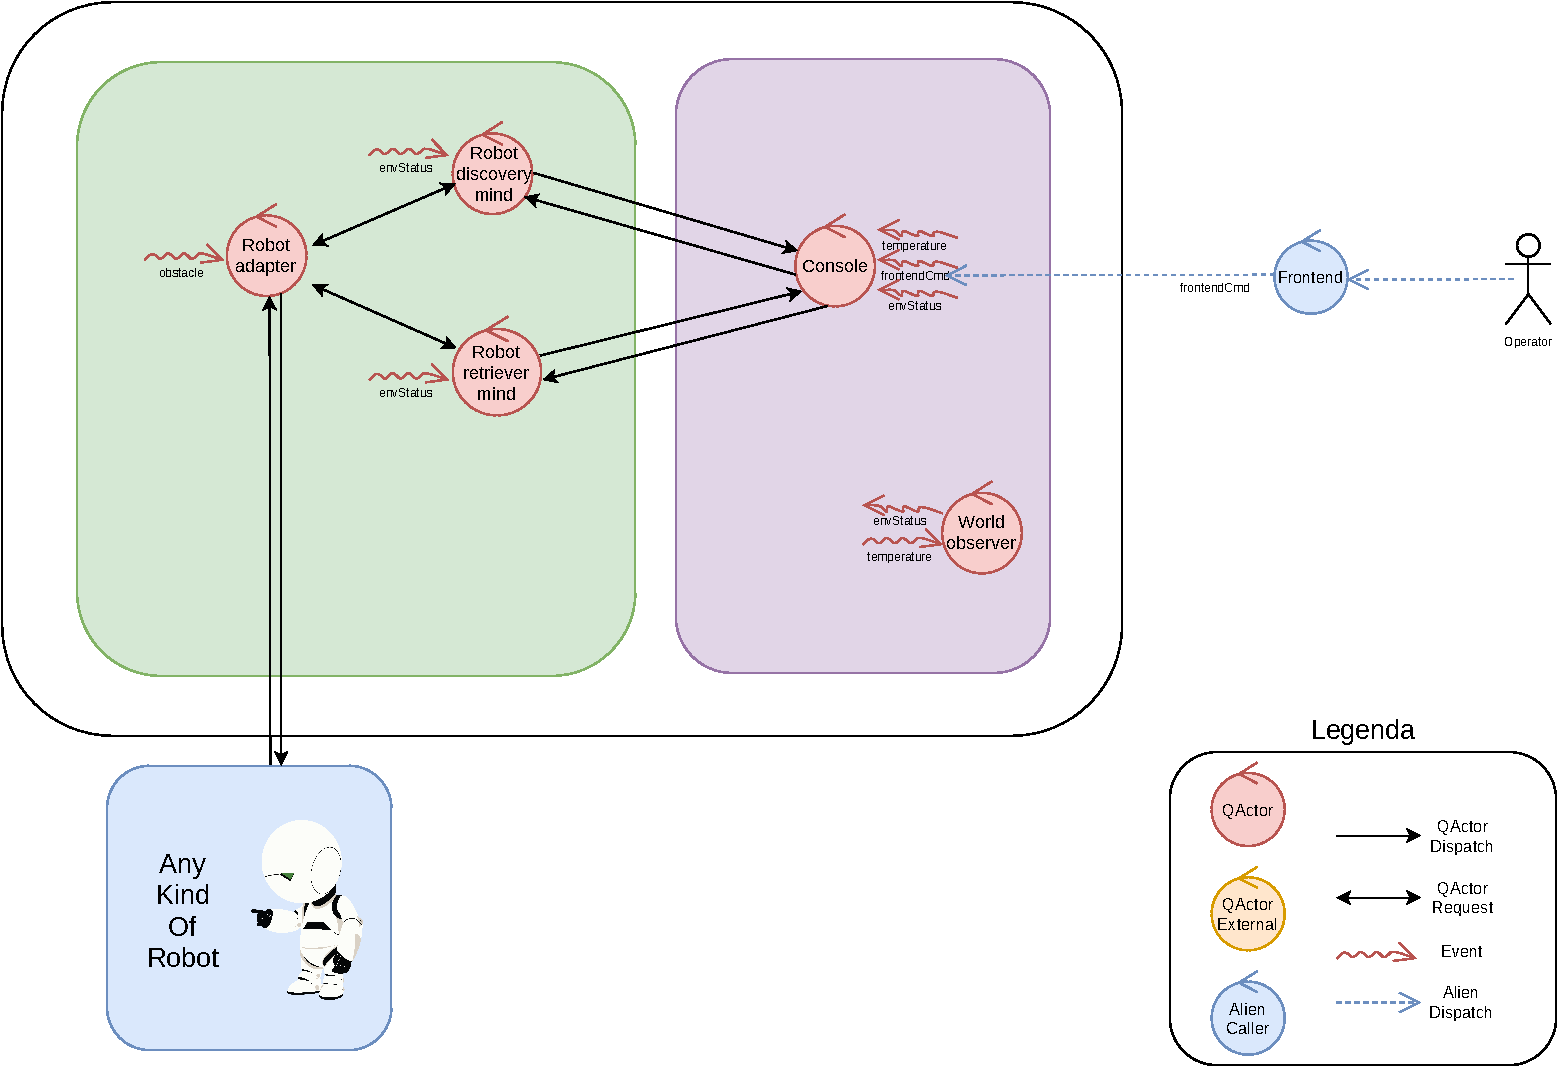
\includegraphics[width=\textwidth]{res/analysis}%
  \caption{Grafico realizzato in draw.io che rappresenta lo stato del sistema in output all'analisi}%
  \label{fig:analysis}
\end{figure}

%===========================================================================
% \subsection{Casi d'uso}\labelssec{use_cases}

% \subsection{Scenario}\labelssec{scenarios}

% \subsection{Modello di dominio}\labelssec{modello}

% \subsection{Test plan}\labelssec{test_plan}

%===========================================================================
% \section{Analisi del problema}\labelsec{problem_analysis}

%===========================================================================
% \subsection{Architettura logica}\labelssec{logic_arch}

% \subsection{Abstraction gap}\labelssec{abstraction-gap}

% \subsection{Analisi del rischio}\labelssec{risk_analysis}

%===========================================================================
% \section{Piano di lavoro}\labelsec{work_plan}

%===========================================================================

%===========================================================================
\section{Progettazione}\labelsec{project}
TODO % TODO
%===========================================================================

% \subsection{Struttura}\labelssec{structure}
% \subsection{Interazione}\labelssec{interaction}
% \subsection{Comportamento}\labelssec{behavior}

%===========================================================================
% \section{Implementazione}\labelsec{implementation}

%===========================================================================

%===========================================================================
% \section{Testing}\labelsec{testing}

%===========================================================================

%===========================================================================
% \section{Deployment}\labelsec{deployment}
%===========================================================================

%===========================================================================
% \section{Manutenzione}\labelsec{maintenance}

%===========================================================================

\newpage

% \section{Difficoltà e note varie}

Durante lo sviluppo, sono state riscontrate diverse difficoltà che per completezza è bene elencare.

Risulta comunque evidente che queste criticità rispecchino il mondo reale e dunque bene si vadano ad integrare con lo scopo di questo progetto di rispecchiare fedelmente un processo di sviluppo all'interno di una software house.

\subsection{Creazione dinamica degli attori}
Sarebbe stato molto utile poter creare dinamicamente gli attori in QA\@:
infatti, sarebbe stato possibile creare un robot adapter per ogni robot a runtime senza dover assegnare tutti i robot usati allo stesso adapter.

Per esempio, sarebbe stato possibile usare un robot per l'esplorazione ed uno differente per il recupero.

\subsection{Tecnologie datate}
Esperienza interessante è stata il dover avere a che fare con tecnologie almeno in parte datate o non complete:

\begin{itemize}
  \item
    come specificato più nel dettaglio in~\Cref{app:raspi},
    l'immagine per Raspberry Pi fornita come riferimento dalla software house è basata su una versione datata dei pacchetti, e la configurazione in parte fuori standard ha convinto a realizzare una nuova immagine al solo scopo di questo progetto.
  \item
    il linguaggio QA è eccezionale sotto il punto di vista della realizzazione di metamodelli e per il \textit{bootstrap} di prototipi, ma come anche da documentazione ci sono alcune funzionalità solo teorizzate o implementate in parte che possono risultare limitanti dal lato pratico.
    \begin{itemize}
      \item
        è comunque importante specificare che è stata usata la versione 1.5.13.2, in quanto quella presentata durante le lezioni e meglio conosciuta;
        è probabile che la nuova versione disponibile possa arginare alcune delle criticità delle versioni più vecchie.
    \end{itemize}
  \item
    la software factory richiede necessariamente Eclipse per la code generation e presenta dunque un lock-in non indifferente rispetto a tecnologie differenti basate su build system (ad esempio, Gradle) anziché su IDE, anche in ottica di continuous integration.
  \item
    il template fornito per realizzare questo report è basato su una versione datata e modificata della classe \LaTeX{} \texttt{LLNCS} fornita da Springer\footnote{\url{https://www.springer.com/gp/computer-science/lncs/conference-proceedings-guidelines}};
    a causa di questo vincolo, sono state riscontrate difficoltà con l'utilizzo di pacchetti moderni (come ad esempio \texttt{subcaption}).
\end{itemize}

\subsection{Modularizzazione del metamodello QA}
Durante lo sviluppo è stata riscontrata una limitazione non indifferente, soprattutto in termini di sintesi e pulizia del codice:
i file QA prodotti tendono a diventare molto grandi (anche più di 700 righe) e diventano di difficile fruizione.

\subsection{Stampa degli errori}
Durante lo sviluppo, un grosso rallentamento è stato causato dalla mancata stampa su console di errori incontrati, poiché ciò rende molto più complesso il debug.

\subsection{MQTT non funzionante}
Durante lo sviluppo sono stati riscontrati diversi problemi con l'uso di MQTT\@:
infatti, la software factory incita l'utilizzo di MQTT per la realizzazione della comunicazione tra le entità in gioco, ma ha grossi problemi di implementazione
\begin{itemize}
    \item pacchetti persi;
    \item problemi durante l'avvio degli attori dovuti ad una sovrapposizione delle connessioni;
    \item ritardo di comunicazione anche su singola macchina in comunicazione tramite localhost.
\end{itemize}
 % TODO

% %% Direttive TeXworks:
% !TeX root = ../report.tex
% !TEX encoding = UTF-8 Unicode
% !TeX spellcheck = it-IT

\begin{appendix}
  \section{Appendice: Immagine del Raspberry Pi}\label{app:raspi}

  La software house metteva a disposizione una immagine della distribuzione Raspbian\footnote{\url{https://www.raspberrypi.org/downloads/raspbian/}}
  (una versione di Debian per Raspberry Pi) adattata dalla software house per l'uso interno.

  L'immagine è però basata su una vecchia versione di Raspbian Jessie datata 26 febbraio 2016 e presenta diversi problemi.
  Già in passato la software house aveva riscontrato problemi e aveva proposto \textit{fix}
  documentati sul sito\footnote{\url{http://htmlpreview.github.io/?https://github.com/anatali/iss2018/blob/master/it.unibo.issMaterial/issdocs/Material/LectureCesena1819.html}}
  della software house.

  La configurazione standard prevede l'accesso alla rete pubblica tramite WiFi e la configurazione locale tramite connessione diretta ethernet;
  poiché la macchina di sviluppo utilizzata non dispone di connessione ethernet, si è deciso,
  consci anche degli altri problemi presenti nell'immagine, di adattare una versione più moderna di Raspbian Buster lite per questo progetto.

  \subsection{Configurazione del Raspberry Pi}\label{app:raspi:conf}

  Si è scelto di utilizzare un modulo WiFi USB in aggiunta a quello integrato nel Raspberry Pi 3,
  ma è possibile utilizzare il solo modulo WiFi integrato sia come access point che come client, pur con maggiori instabilità e minori velocità.

  La procedura di adattamento dell'immagine è stata documentata in modo da poter essere riproducibile in futuro.

  \begin{enumerate}
    \item
      La base dell'immagine è l'ultima versione di \textbf{Raspbian} nella sua versione minimale \textbf{lite}:
      in questo caso, la versione Buster del 26 settembre 2019;
    \item
      l'immagine è stata connessa alla rete tramite WiFi e i pacchetti sono stati aggiornati tramite \texttt{apt};
    \item
      seguendo la documentazione fornita sul sito ufficiale\footnote{\url{https://raspap.com/}},
      è stato installato \textbf{RaspAP} e configurato per funzionare esclusivamente via WiFi:
      \begin{enumerate}
        \item
          \texttt{curl -sL https://install.raspap.com | bash} permette di installare RaspAP\@;
        \item
          seguendo le FAQ\footnote{\url{https://github.com/billz/raspap-webgui/wiki/FAQs\#can-i-use-wlan0-and-wlan1-rather-than-eth0-for-my-ap}}
          al file \texttt{includes/config.php} si è aggiunta \texttt{wlan1} come client interface e si è impostato nel file \texttt{/etc/dhcpcd.conf}
          \texttt{wlan0} come access point
      \end{enumerate}
      In questo modo, il dispositivo dovrebbe essere in grado di collegarsi alla rete WiFi pre-configurata e mettere a disposizione una rete con SSID ``raspi-webgui''.
    \item
      utilizzando lo script ufficiale\footnote{\url{https://github.com/docker/docker-install}}
      (ma si sarebbe potuta seguire la documentazione\footnote{\url{https://docs.docker.com/install/linux/docker-ce/debian/}}), si è installato Docker;
    \item
      si è installato Java 1.8 tramite pacchetto \texttt{openjdk-8-jdk-headless};
    \item
      il broker MQTT Mosquitto viene eseguito tramite container Docker\footnote{\url{https://hub.docker.com/_/eclipse-mosquitto}}.
  \end{enumerate}
\end{appendix}
 % TODO

\end{document}
